\chapter{計算実験}\label{computational_result}
\section{計算環境}
実験に用いるプログラムはPythonを用いて実装し, 計算機はMacBookAir2020 (CPU: 8 コア Apple M1 chip, メモリ: 8 GB LPDDR4)を用いて行った. 

\section{第一段階の求解結果}
整数計画ソルバー (Gurobi Optimizer ver. 9.5)を用いて計算した結果, 全ての問題例で最適解が得られた. 
出力の例を図\ref{first-no-rei}に示す. 
長方形内の番号はグループの番号を表す. 
灰色の長方形は, ランプを表す. \\

\begin{figure}[b]
    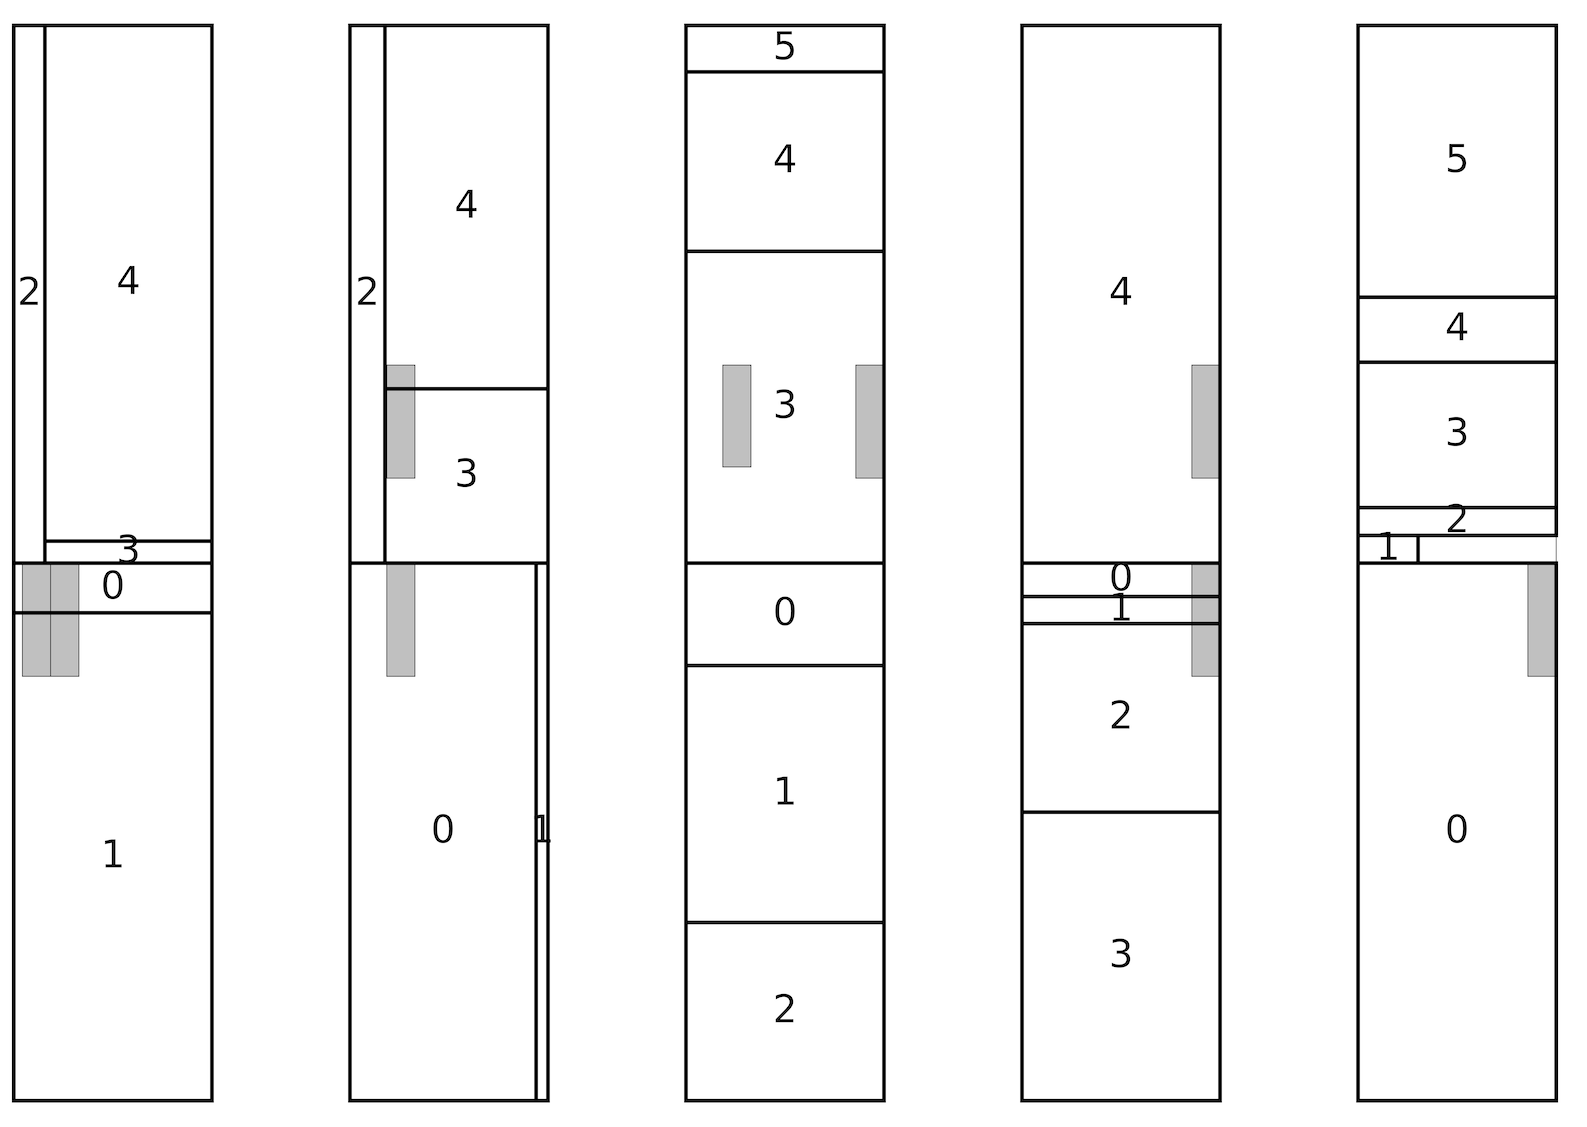
\includegraphics[scale=0.3, bb = 0 0 1 1]{5-first-no-rei.png}
    \caption{第一段階の出力の例}
    \label{first-no-rei}
\end{figure}
\clearpage

\section{第二段階の求解結果}
出力される配置図の例を図\ref{second-no-rei}に示す. 
各長方形が車を表し, 色は積み地の種類を表す. \\

\begin{figure}[b]
    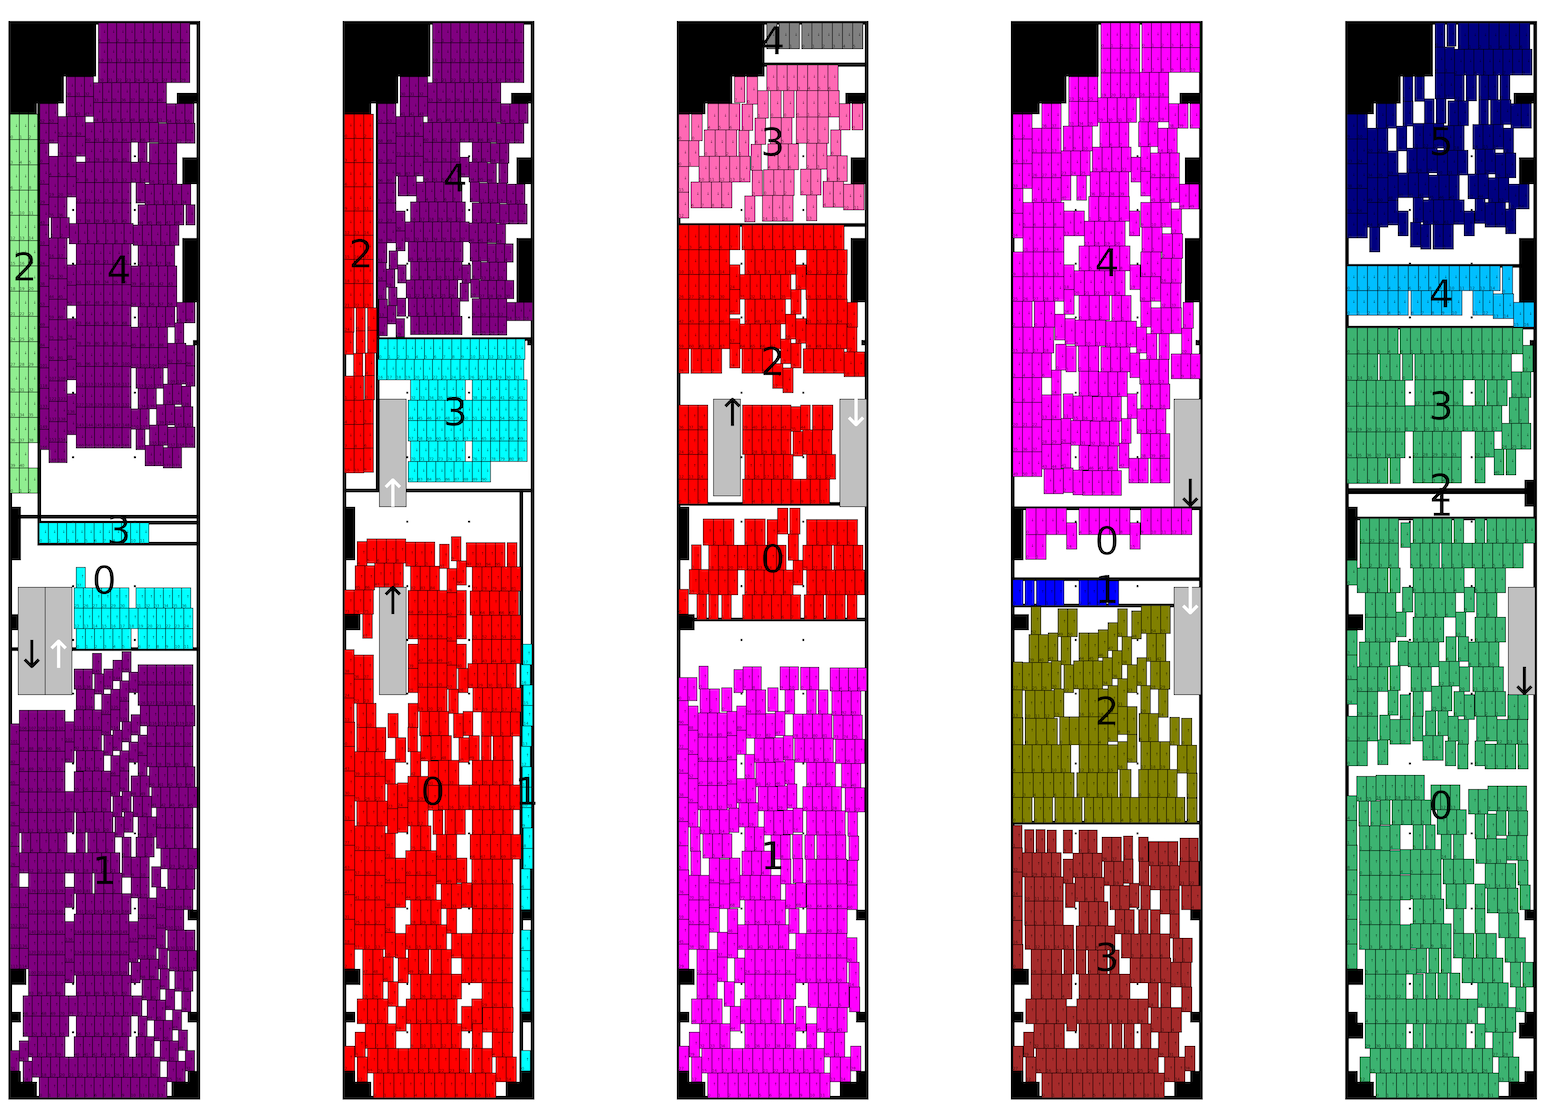
\includegraphics[scale=0.3, bb = 0 0 1 1]{5-second-no-rei.png}
    \caption{第二段階の出力図の例}
    \label{second-no-rei}
\end{figure}

\section{局所探索法による解の改善}
以下の表\ref{review-local}に局所探索法を加えることで詰め込むことのできた解の改善結果を示す. 
表の台数は詰め込むことのできた車の数を表す. 

\begin{table}[htbp]
    \centering
    \caption{近傍操作による解の改善}
    \label{review-local}
    \begin{tabular}{ccccccc}
    \hline
    \multicolumn{2}{c}{問題例}                               & \multicolumn{1}{l}{} & \multicolumn{2}{c}{初期解}                           & \multicolumn{2}{c}{局所探索}                          \\
    \hline
    \multicolumn{1}{l}{問題番号} & \multicolumn{1}{l}{台数} & \multicolumn{1}{l}{} & \multicolumn{1}{l}{台数} & \multicolumn{1}{l}{計算時間} & \multicolumn{1}{l}{台数} & \multicolumn{1}{l}{計算時間} \\
    \hline
    1                        & 773                        &                      & 753                    & 142                      & 765                    & 447                      \\
    2                        & 604                        &                      & 534                    & 274                      & 572                    & 618                      \\
    3                        & 594                        &                      & 554                    & 271                      & 560                    & 583                      \\
    4                        & 481                        &                      & 459                    & 233                      & 481                    & 414                      \\
    5                        & 276                        &                      & 593                    & 276                      & 592                    & 395                     \\
    \hline
    \end{tabular}
    \end{table}
